\chap{Discussion}

 The purpose of this chapter is to provide some additional considerations and the author's own reflections on the methods and their limitations, which has not already been covered in the previous sections.

\sect{Physiological binning when using the golden angle}
The golden angle provides an approximately uniform distribution of k-space readouts for an arbitrary number of readouts. This means that an arbitrary number of readouts will provide a good k-space coverage, as opposed to linear radial methods, which would require an \emph{a priori} decision regarding the number of readouts. The idea is that every new line will provide additional k-space coverage where it is most needed, i.e. each succeeding readout will fill one of the largest gaps in k-space. This has sometimes been interpreted to mean that an arbitrary non-continuous subset of readouts will constitute a uniform k-space coverage. If the number of readouts is large, it could be expected that a \textbf{random} subset is near uniform if readouts are chosen with equal probability. However, in real applications, we are rarely interested in random subsets. Rather, we use some physiological motion signal, such as an ECG or respiratory signal to select readouts. Such functions are often periodic to some degree, meaning that we periodically discard and reject readouts. This tends to create gaps in the sampling pattern, resulting in severe image artifacts, see Figure~\ref{fig:swig_binning}.
\begin{figure}[htbp]
    \centering
    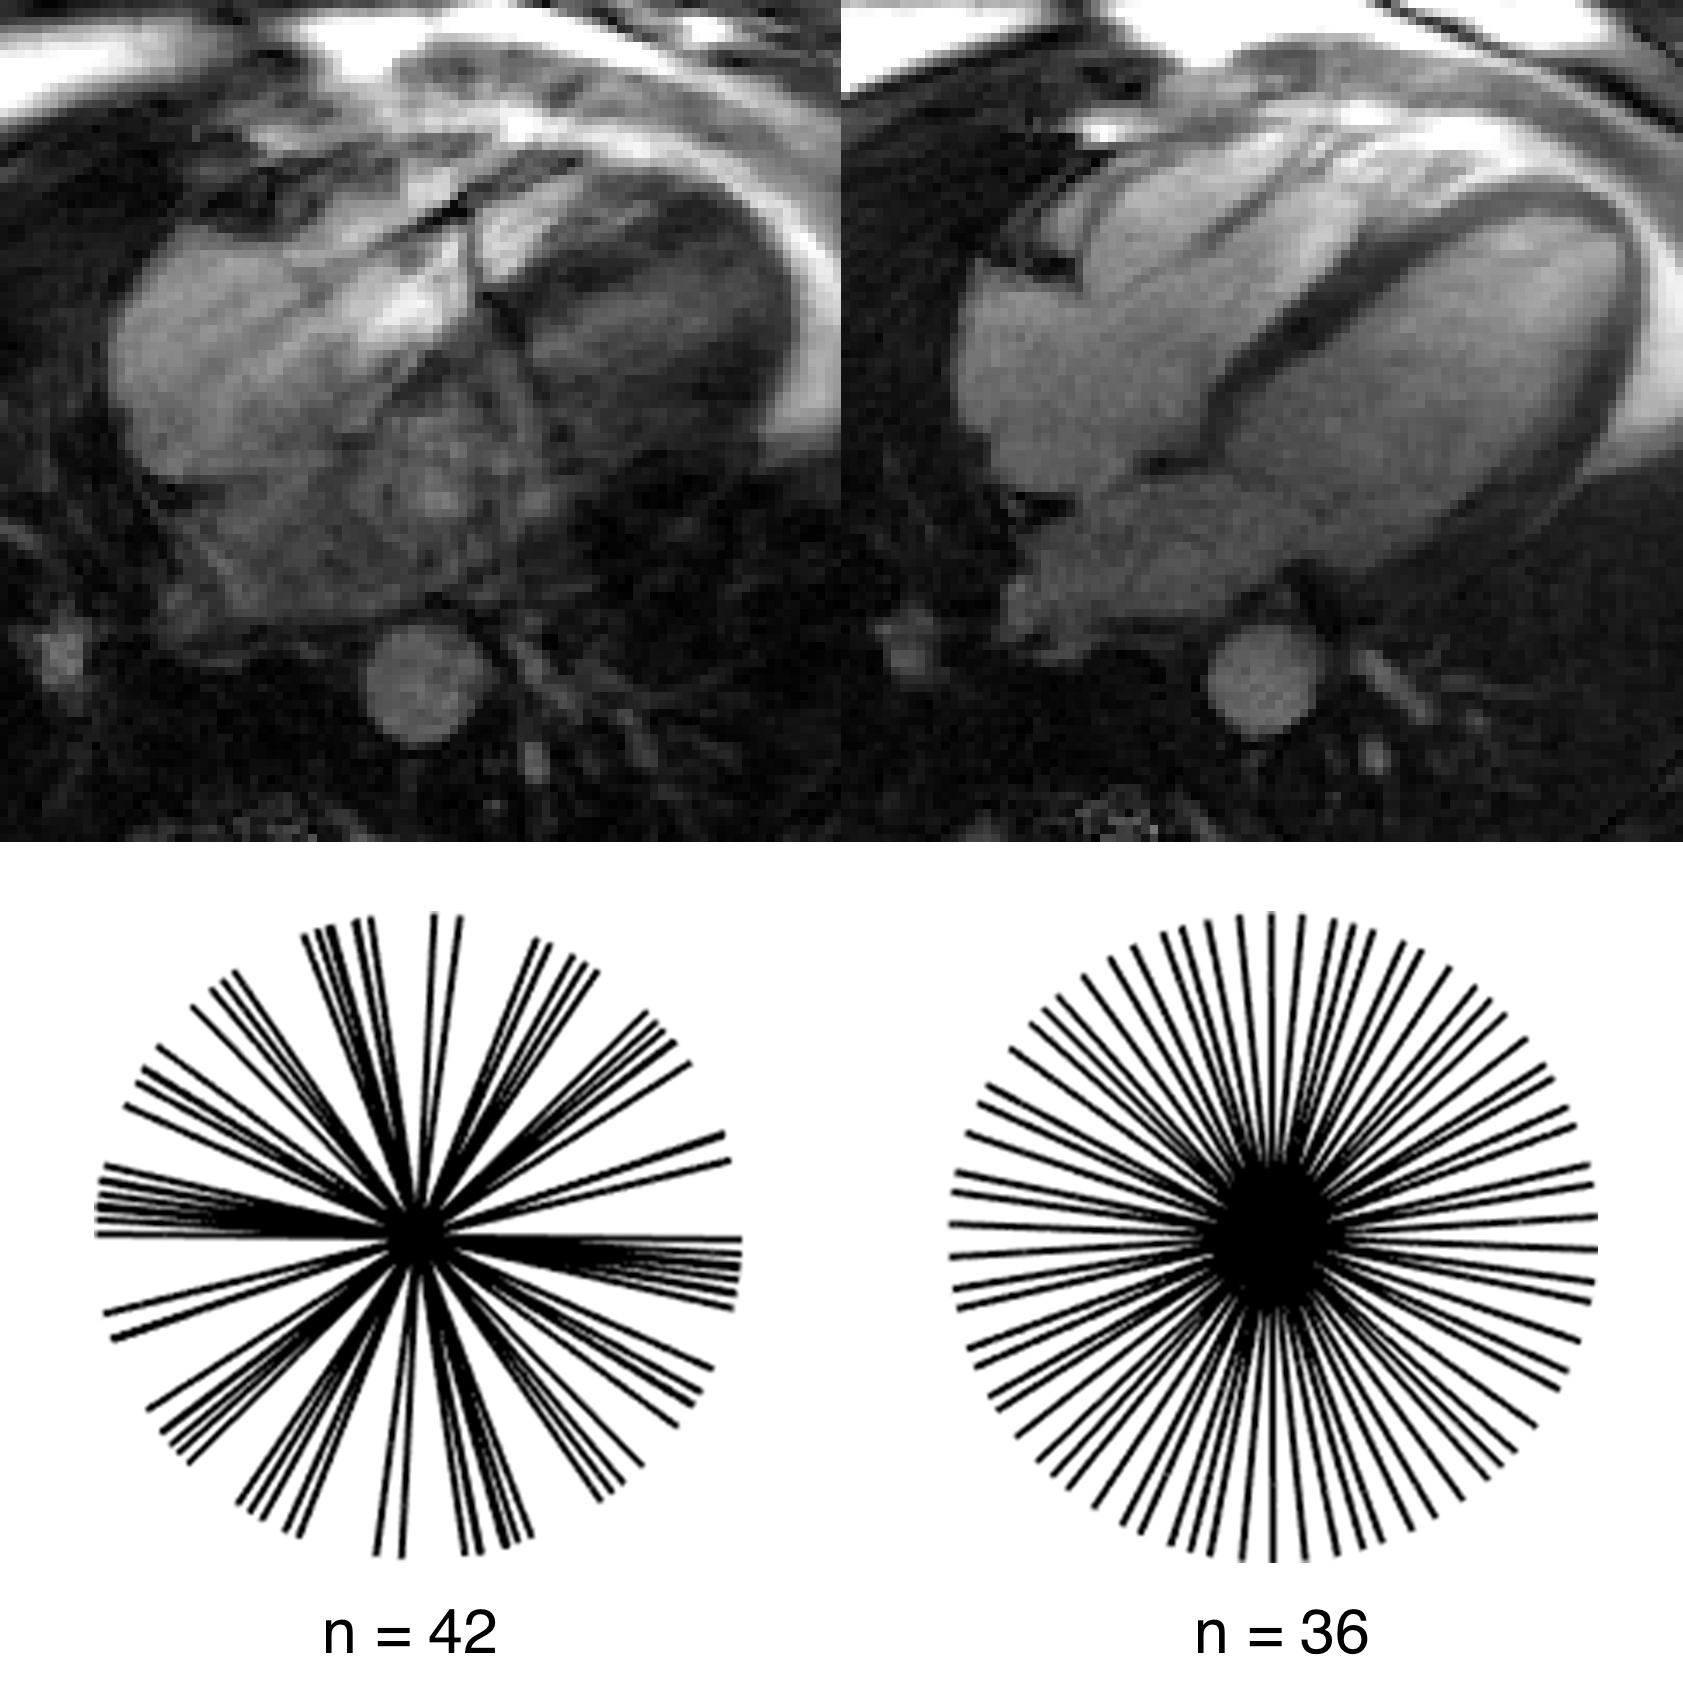
\includegraphics[width=0.75\textwidth]{with_traj.png}
    \caption{Examples of ECG-binning of the conventional golden-angle profile ordering (left) and the 2D-SWIG profile ordering (right).}
    \label{fig:swig_binning}
\end{figure}
Using the SWIG method, we can adapt the sampling to a physiological signal, such as the ECG, as described in this thesis, but in theory, it should be possible to adapt the acquisition to any motion signal that we can acquire at imaging time. Recent research has lead to the development of the Doppler ultrasound (DUS) \Nomenclature{DUS}{Doppler ultrasound} gating device for fetal cardiac gating~\cite{Kording2018}. Such a device could potentially also be used to prospectively measure respiratory motion, enabling multidimensional SWIG-imaging.

\sect{Underestimation of transmitral blood flow using SWIG-PC}
One of the findings in \textbf{Study III} was that SWIG agrees with Doppler echocardiography for myocardial tissue velocity measurements, but that the transmitral blood flow velocity were underestimated. This finding is surprising, as the myocardial tissue velocities were expected to be a more challenging target with regards to accuracy. The myocardial velocity peak in the early filling (e') is very narrow, so a low temporal footprint is expected to be needed in order to capture the peak velocity accurately. The velocity peaks in the transmitral blood flow are much broader, so such a high temporal resolution should not be needed. Yet the results clearly show a systematic underestimation of the transmitral blood flow. While more work is warranted, a possible explanation for this is that the slice planning was sub-optimal. Recent work has proposed slice tracking for phase~contrast imaging of the valves~\cite{Seemann2019}, which is a method that could potentially be adopted into the SWIG-PC method. Another possible solution would be to, instead of planning in a short-axis orientation, use a long-axis image with in-plane velocity encoding, where the active measurement volume could be placed in an optimal position to capture the transmitral inflow. 

\sect{Limitations}
This thesis would not be complete without a reflection on its limitations. 

In \textbf{Study I}, the sample size was limited and comprised mainly health volunteers. A more systematic evaluation would be necessary to determine the clinical utility of the method. Preferably with paired evaluations between CTA and MRI, to be able to estimate the sensitivity and specificity of each method. Another important methodological limitation is the blinding of the observers who were asked to score the images. When comparing a Cartesian and radial method, it is hard to blind the observer to the method, as radial images often has a very characteristic look. A possible solution could have been to calculate a mask outside of the body to hide the streaks in the air, which may be the biggest giveaway and, at the same time, contributing little to the utility of the images.
In \textbf{Study II}, a major limitation was the lack of systematic evaluation of the method \emph{in vivo}, as only a single subject was imaged. Another important limitation that should be mention is that k-space uniformity could have been a confounding factor. The hypothesis was that the improved image quality was due to reduced angular differences within a 2-TR phase cycle. However, as the sampling trajectory was changed, this could also have affected the sampling uniformity and thereby the image quality. It may have been useful to use an external measure, such as a field camera, in an attempt to quantify how much of the improvement came from the reduced angular switching.
In \textbf{Study III}, tissue velocity measurements were compared between CMR and Doppler echocardiography. Initial results from the pilot study suggested that the CMR overestimated tissue velocities compared to Doppler echocardiography. However, no comparisons were made to a gold standard. A suitable gold standard for simultaneous evaluation of both measurements could have been ultrasonic micrometry \cite{Kokubo1995}.
In \textbf{Study IV}, a major limitation was the lack of systematic evaluation \emph{in vivo}. As the images were reconstructed using a compressed sensing algorithm with temporal regularization, it is important to verify that temporal smoothing did not affect the measurement of ventricular volumes. This could have been verified against measurements of the ventricular volumes using breath-held two-dimensional cine.

A limitation for all studies involving healthy volunteers was that volunteer recruitment was made mostly through the author's own network of contacts, and many volunteers were either researchers or medical professionals. This may have contributed to some systematic bias, as most volunteers were young and of above-average fitness, as opposed to the typical patient referred for cardiac MRI.

\sect{Ethical considerations}
Most of the thesis involved some degree of development of novel clinical methods. As such, they have to ultimately be evaluated in human subjects, both healthy volunteers and patients. All studies which involved human subject were performed in accordance with the Declaration of Helsinki~\cite{WMA2013}.

\subsect{Healthy volunteers}
Ethical permits were in place for evaluating the methods, both for healthy volunteers and patients. It is important to note that there existed dedicated ethical approval to test all methods in both healthy volunteers and patients, as there may exist situations where it may be ethical to evaluate a method in a patient but not a healthy volunteer.
All volunteers gave informed, written consent to participate. Their personal information was treated confidentially as required by both ethical guidelines and the law. Most of the research in these studies were performed on raw k-space data. Consequently, the data could be anonymized, i.e., irreversibly separated from any identifying information.

\subsect{Patients}
In the studies which involved patients, all necessary steps were taken to ensure their privacy and integrity. The patients involved in \textbf{Study I} were prospectively included based on their clinical referral. In \textbf{Study II}, no patients were involved. In \textbf{Study III} and \textbf{Study IV}, patients were retrospectively included from the body of patients that had agreed to have their data used for clinical research. In the case of the prospectively included patients, their decision to participate meant that they were subject to an additional MRI scan. Importantly, this did not delay the care they would have received had they not chosen to participate. In the case of retrospectively included patient, their participation did not alter the clinical care they received in the healthcare system.

\sect{Safety}
MRI is a non-invasive method of imaging that does not expose the subject to ionizing radiation. As such, MRI should be considered a safe imaging modality. No long-term biological effects have been associated with MRI. The short-term effects experienced by some patients may include claustrophobia, magnetophosphenes (an optical illusion where the subject experiences light flashes), peripheral nervous stimulation, and heating. None of the research protocols included contrast agents or other drugs. In cases where patients received a contrast agent, this was part of the clinical routine and administered by a trained professional. None of the scanner's safety features were disengaged during the scanning of patients and healthy volunteers, and the most recent safety guidelines were followed at all times~\cite{Kanal2013,Greenberg2020}.

\sect{Future perspectives}
Although golden-angle based methods have been around since 2007, they have yet to find mainstream adoption. There is still a strong bias towards conventional Cartesian methods. Many sequence development environments, and image reconstruction tools have not yet adapted to advanced sampling techniques, and the vendors have not always caught up with the latest research. However, the research community have taken it upon themselves to develop sequence programming environments~\cite{Layton2017,Skare2017:ISMRM}, and open-source image reconstruction toolboxes such as BART~\cite{Uecker2015:ISMRM} and Gadgetron~\cite{Hansen2013}, which can be integrated into the scanner workflow and even enable online image reconstruction in the cloud~\cite{Xue2015}.

An elusive target has for long been the ``five minute MRI'', i.e., to perform a comprehensive cardiac MRI examination in five minutes, as opposed to 45 minutes or even an hour, which is the norm today. Professor Daniel K. Sodickson, at NYU Langone Health, has spoken about a future where the patient goes in the scanner, and data is continuously acquired. When the patient has left, powerful computational computers are put to work, or leveraging the power of the cloud, to process the data and create the imaging slices and contrasts needed for the clinical diagnosis. Further along, machine learning might directly analyze the images in some other feature space, and not necessarily as images. Major advances in machine learning are already underway with the advent of the AutoMAP-method~\cite{Zhu2018}, which learns domain transfer from the k-space to the image domain using neural networks and can in the process learn to compensate for image artifacts. Both the AutoSEQ~\cite{Zhu2018:ISMRM} and MRZero~\cite{Loktyushin2020} methods have taken things a step further. Both are using Bayesian reinforcement learning to learn pulse sequences generation without user interaction. Golden-angle based methods may very well play a part in these developments, as they are particularly suited for volumetric imaging, and their golden nature lends itself to continuous sampling where each new readout will provide unique information. With the aforementioned developments in terms of sequence development environments, reconstruction algorithms, and more readily available compute power, it is likely that non-Cartesian methods will have an essential place in the future for cardiovascular MRI.